\documentclass[10pt,twocolumn,letterpaper]{article}

\usepackage{cvpr}
\usepackage{times}
\usepackage{epsfig}
\usepackage{graphicx}
\usepackage{amsmath}
\usepackage{amssymb}
\usepackage{multirow}
\usepackage{caption}
\usepackage{subcaption}
\usepackage{url}
\graphicspath{{./images/helper/}{./images/apple2orange/}{./images/summer2winter/}
{./images/arial2times/}{./images/arial2times_word/}}

\newcommand{\norm}[1]{\left\lVert#1\right\rVert}
\newcommand{\normm}[1]{\left\lVert\lVert#1\right\rVert\rVert}

% Include other packages here, before hyperref.

% If you comment hyperref and then uncomment it, you should delete
% egpaper.aux before re-running latex.  (Or just hit 'q' on the first latex
% run, let it finish, and you should be clear).
\usepackage[breaklinks=true,bookmarks=false]{hyperref}

\cvprfinalcopy % *** Uncomment this line for the final submission

\def\cvprPaperID{****} % *** Enter the CVPR Paper ID here
\def\httilde{\mbox{\tt\raisebox{-.5ex}{\symbol{126}}}}

% Pages are numbered in submission mode, and unnumbered in camera-ready
%\ifcvprfinal\pagestyle{empty}\fi
\setcounter{page}{1}
\hypersetup{draft}
\begin{document}

%%%%%%%%% TITLE
\title{Exploring CycleGAN and Its Application to Font Transfer}

\author{Asif Iqbal\\
Ryerson University\\
Toronto, ON, Canada\\
{\tt\small asif1.iqbal@ryerson.ca}
% For a paper whose authors are all at the same institution,
% omit the following lines up until the closing ``}''.
% Additional authors and addresses can be added with ``\and'',
% just like the second author.
% To save space, use either the email address or home page, not both
%\and
%Second Author\\
%Institution2\\
%First line of institution2 address\\
%{\tt\small secondauthor@i2.org}
}

\maketitle
%\thispagestyle{empty}

%%%%%%%%% ABSTRACT
\begin{abstract}
   Unpaired image to image translation has gained quite a bit of attention with the advent of Cycle-Consistent Generative Adversarial Networks (CycleGANs). Translation domains like $horse \leftrightarrow zebra$, $apple \leftrightarrow orange$, $photo \leftrightarrow painting$, $summer \leftrightarrow winter$ and several others have been explored in the original work. In this paper, we plan to regenerate some of the works done in CycleGAN, try out a couple of the already tried domains on our own, and finally apply the CycleGAN concept to font style transfer. Specifically, we try it out on Arial to Times New Roman black fonts for single uppercase characters and also on lowercase multi-character words, and demonstrate that it might be a promising direction. Although it is not at all hard to get paired data for text fonts, we hope that our approach can in the future be extended to font image transfer tasks where paired data might indeed be hard to attain. The code has been made open source in the Github repository \href{https://github.com/asif31iqbal/cycle-gan-pytorch}{https://github.com/asif31iqbal/cycle-gan-pytorch}.
\end{abstract}

%%%%%%%%% BODY TEXT
\section{Introduction}
Image-to-image translation is a class of vision and graphics problems where the goal 
is to learn the mapping between an input image and an output image using a training 
set of aligned image pairs \cite{cyclegan}. Image to image \cite{cyclegan}. The field 
of image-to-image translation has been studied to quite an extent over the last couple 
of years. This problem can be more broadly described as converting an image from 
one representation of a given scene, $x$, to another, $y$, e.g., grayscale to color, 
image to semantic labels, edge-map to photograph \cite{pix2pix, cyclegan}. Years 
of research in computer vision, image processing, computational photography, 
and graphics have produced powerful translation systems in the supervised setting, 
where example image pairs $\{x_i , y_i\}_{i=1}^N$ are available \cite{rel1, rel2, rel3, 
rel4, rel5, rel6, rel7, rel8, rel9, rel10}. However, obtaining paired data for many 
tasks can be difficult and expensive. Obtaining input-output pairs for graphics 
tasks like artistic stylization can be even more difficult since the desired output 
is highly complex, typically requiring artistic authoring \cite{cyclegan}. Let's say 
we want to transfer a particular summer scene into a winter one and vice versa. 
We can easily imagine how the corresponding winter version of a summer scene 
or a summer version of a winter scene might look like even though we might have 
never seen a summer and winter version of the same scene side by side. Based on 
this insight, the authors of CycleGAN \cite{cyclegan} came up with the algorithm 
that can learn to translate between domains without paired input-output examples, 
assuming that there is some underlying relationship between the domains – for 
example, that they are two different renderings of the same underlying scene – and seek to learn that relationship. Although the algorithm lacks supervision in the form 
of paired examples, it can exploit supervision at the level of sets: we are given one 
set of images in domain $X$ and a different set in domain $Y$. We may train a mapping 
$G : X \leftarrow Y$ such that the output $\hat{y} = G(x)$, $x \in X$, is indistinguishable from 
images $y \in Y$ by an adversary trained to classify $\hat{y}$ apart from $y$ \cite{cyclegan}. However,
as discussed in \cite{cyclegan} that there could be infinitely many mappings $G$ that will induce the same distribution over $\hat{y}$. Also, there is the problem of mode collapse \cite{gan1}, where all input images map to the same output image and the optimization fails to make progress.

To tackle these problems, the CycleGAN \cite{cyclegan} authors leverage the notion of \textit{cycle consistency}, in the sense that if we transfer the font style of a character from Arial to Times New Roman, and then translate it back from Times New Roman to Arial, we should get back the original character. Mathematically, if we have a translator $G : X \leftarrow Y$ and another translator $F: Y \leftarrow X$, then G and F should be inverses of each other, and both mappings should be bijections. We apply this structural assumption by training both the mapping G and F simultaneously, and adding a cycle consistency loss \cite{rel21} that encourages $F(G(x)) \approx x$ and $G(F(y)) \approx y$.

The authors \cite{cyclegan} have applied this idea to a wide range of
applications, like collection style transfer, object transfiguration, season
transfer and photo enhancement. In this paper, we first attempt to regenerate
their work and network architecture from scratch, apply it to couple of domains 
that they have already tried out, namely season ($summer \leftrightarrow winter$) 
transfer and object style transfer ($apple \leftrightarrow orange$). Next, we apply 
it to the domain of font style transfer. We limit ourselves to just two fonts - Arial and 
Times New Roman. We try it on single uppercase black English characters and on 
lowercase black English words. Although it is not difficult to get paired data for this 
sort of font style transfers for well known fonts which are widely available, there are 
unknown fonts, text and calligraphy styles that are available in the wild (like is posters or artistic
drawings) for which it is 
not easy to get paired data and applying the CycleGAN concept might be a good idea. 
The attempt with known fonts in this paper is a baby step towards the possible 
applicability of unknown font style transfers using cycle consistency.

\section{Related Work}
Over the last couple of years, Generative Adversarial Networks (GANs) \cite{gan1, gan2} have achieved
quite a bit of success in image generation. The key idea behind GAN's success is the \textit{adversarial 
loss} that forces the generated image to be indistinguishable from the input image. In the CycleGAN case,
the adversarial loss has been adopted in such a way that the generated images are indistinguishable from 
the images in the target domain.

Much of the related work regarding unpaired image-to-image translation have been mentioned in the 
original paper \cite{cyclegan}. Approaches like \cite{rel3, rel6, rel11, rel12} and \textbf{Pix2Pix} work on 
paired training examples, as opposed to the unpaired training concept that CycleGAN relies on.

There has been a few works on unpaired image-to-image translation as well. Works like \cite{rel13, rel14, 
rel15} uses a weight sharing strategy between domains. Another group of work like \cite{rel16, rel17, rel18} 
encourages the input and output to share specific content features even though they may differ in style. 
Unlike these approaches, the CycleGAN concept does not rely on any task specific, predefined similarity 
measurements. It's more of a general purpose framework.

As mentioned in the original paper, the idea of cycle consistency also has quite a bit of a history. Of these 
works, \cite{rel19}, \cite{rel20} and \cite{rel21} are the ones that are conceptually most similar to 
CycleGANs.

Neural Style Transfer \cite{rel4, rel22, rel23} is another family of work for image to image translation, 
which synthesizes an image by combining the content of one image with the style of another image. 
Again, this is a paired training concept while CycleGAN is unpaired.

The primary focus of CycleGAN and hence also of this paper, is learning the mapping between two two image collection, rather than between two specific images, by trying to capture correspondence between higher-level appearance structures. We try to apply the same idea in case of font style transfer.

There has been use of GANs specifically in font style transfer as well. The most important one seems to be
the use of multi-content GAN \cite{gan3}. However, their main focus is taking partial observations of highly-
stylized text and generalizing the observations to generate unobserved fonts. Our intent, however, in this paper is to apply the general framework of cycle consistency to font style transfer.

In the remainder of this paper, we discuss the problem formulation, data collection, network architecture
and experimentation in order.

\section{Problem Formulation}

We formulate our problem in the same way the original authors \cite{cyclegan} did, where the goal is to 
learn mapping between two domains $A$ and $B$ given training samples $\{a_i\}_{i=1}^N$ where $a_i \in 
A$ and $\{b_j\}_{j=1}^M$ where $b_j \in B$. The problem formulation has been depicted broadly in Figure 
\ref{fig:problem}.

\begin{figure*}[!htb]
     \centering
     \begin{subfigure}[b]{0.4\textwidth}
         \centering
         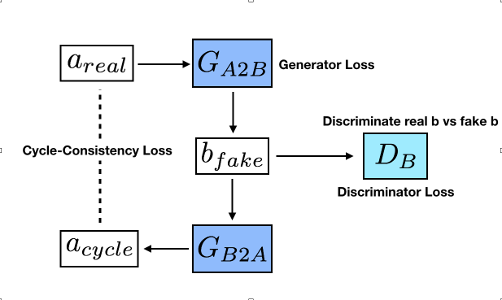
\includegraphics[width=\textwidth]{gan_b}
         \caption{Generator $G_{A2B}$ takes an image $a_{real}$ from domain $A$ and outputs $a_{fake}$ which Discriminator $D_B$ tries to distinguish from actual images in domain $B$. Image $a_{fake}$ is then passed onto generator $G_{B2A}$ which generates $a_{cycle}$. This is used for calculating the \textit{cycle-consistency} loss.}
         \label{fig:gan_b}
     \end{subfigure}
     ~
     \begin{subfigure}[b]{0.4\textwidth}
         \centering
         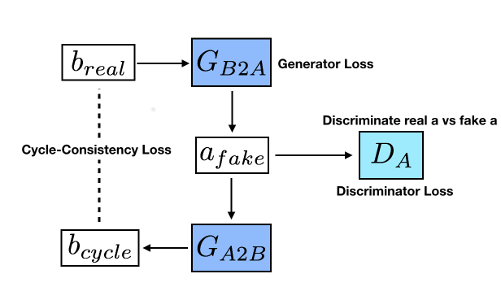
\includegraphics[width=\textwidth]{gan_a}
         \caption{Generator $G_{B2A}$ takes an image $b_{real}$ from domain $B$ and outputs $a_{fake}$ which Discriminator $D_A$ tries to distinguish from actual images in domain A. Image $b_{fake}$ is then passed onto generator $G_{A2B}$ which generates $b_{cycle}$. This is used for calculating the \textit{cycle-consistency} loss.}
         \label{fig:gan_a}
     \end{subfigure}
        \caption{Problem Formulation}
        \label{fig:problem}
\end{figure*} 

We have two generators $G_A$ and $G_B$, and two discriminators $D_A$ and $D_B$. $G_{A2B}$ takes a real 
image $a_{real}$ from domain $A$ and generates a fake image $b_{fake}$ in domain $B$, while $G_{B2A}$ 
takes a real image $b_{real}$ from domain $B$ and generates a fake image $a_{fake}$ in domain $A$. 
Discriminator $D_A$ tries to discriminate between the generated image $a_{fake}$ and real images in 
domain $A$, while discriminator $D_B$ tries to discriminate between the generated image $b_fake$ and 
real images in domain $B$. The generated fake image $b_{fake}$ is then fed back to $G_{B2A}$ to 
generate an image $a_{cycle}$ in domain $A$, while the generated fake image $a_{fake}$ is then fed back 
to $G_{A2B}$ to generate an image $b_{cycle}$ in domain $B$. 

\subsection{Loss Functions}
As can be seen from Figure \ref{fig:problem}, there are broadly 2 sorts of losses - \textit{adversarial 
loss} (generator loss and discriminator loss) and \textit{cycle-consistency loss}. The adversarial loss 
comprises of the losses incurred from the generators trying to fool the discriminators to take fake 
images as real in their corresponding domain, and from the discriminators trying to distinguish fake 
images from real ones. As discussed in \cite{cyclegan}, with large enough capacity, a network can map 
the same set of input images to any random permutation of images in
the target domain, where any of the learned mappings can
induce an output distribution that matches the target distribution.
Thus, adversarial losses alone cannot guarantee
that the learned function can map an individual input $a_{real}$
to a desired output $y_{fake}$. This is where the \textit{cycle-consistency} loss kicks in - the image 
$a_{cycle}$ should be the same as image $a_{real}$, and the image $b_{cycle}$ should be the same as 
image $b_{real}$.

To be complete, the loss functions can be broken down into the following components:

\begin{enumerate}
\item $D_A$ must approve all the original images $a_{real}$ of the domain $A$
\item $D_A$ must reject all the images $b_{fake}$ which are generated by $G_{B2A}$ to fool it
\item $G_{B2A}$ must make $D_A$ approve all the generated images $b_{fake}$, so as to fool it
\item Image $b_{cycle}$ must retain the property of original image $b_{real}$
\item $D_B$ must approve all the original images $b_{real}$ of the domain $B$
\item $D_B$ must reject all the images $a_{fake}$ which are generated by $G_{A2B}$ to fool it
\item $G_{A2B}$ must make $D_B$ approve all the generated images $a_{fake}$, so as to fool it
\item Image $a_{cycle}$ must retain the property of original image $a_{real}$
\end{enumerate}

In the above list, items $1, 2, 3, 5, 6$ and $7$ are adversarial components of the loss, while items 
$4$ and $8$ a re the \textit{cycle-consistency} components.

The original authors used $L_2$ (MSE) loss for the adversarial components, and $L_1$ loss for the 
\textit{cycle-consistency} component since it earned them better results. We adhere to the same 
principle for our work. The loss equations can be mathematically written as follows:

\begin{align*}
\begin{split}
	\mathcal{L}_{disc} ={}& \norm{D_A(a_{real}) - 1}_2 + \norm{D_B(b_{real}) - 1}_2 + \\
							   	     & \norm{D_A(a_{fake}) - 0}_2 + \norm{D_B(b_{fake}) - 0}_2\\ 
\end{split}
\end{align*}

This captures 1, 2, 5 and 6 above.\\

$\mathcal{L}_{gen} = \norm{D_A(a_{fake}) - 0}_2 + \norm{D_B(b_{fake}) - 0}_2$ \\

This captures 3  and 7 above.\\

$\mathcal{L}_{cycle} = \norm{a_{real} - a_{cycle}}_1  + \norm{b_{real} - b_{cycle}}_1$ \\ 

This captures 4 and 8 above.\\

So the total loss comes down to:


$\mathcal{L}_{total} =\mathcal{L}_{disc} + \mathcal{L}_{gen} +	   
                       \lambda\mathcal{L}_{cycle}$


where $\lambda$ is a parameter to control how much weight we want to put on the \textit{cycle-consistency} as opposed to the adversarial behaviour.

In addition, for certain domains, the original authors \cite{cyclegan} also used an \textit{Identity} loss, to ensure that passing an image in domain $A$ through generator $G_{B2A}$ produces the same image and passing an image in domain $B$ through generator $G_{A2B}$ produces the same image.

\begin{align*}
\begin{split}
\mathcal{L}_{identity} ={}&\norm{G_{B2A}(a_{real}) - a_{real}}_1  + \\
						  &\norm{G_{A2B}(b_{real}) - b_{real}}_1 \\ 
\end{split}
\end{align*}

We can control this loss using another parameter $\beta$. In that case, the total loss comes down to:\\

$\mathcal{L}_{total} = \mathcal{L}_{disc} + \mathcal{L}_{gen} + \lambda\mathcal{L}_{cycle} + \beta\mathcal{L}_{identity}$

The original paper uses a $\lambda$ value of 10 and a $\beta$ value of 5 where used.
We keep the $\beta$ value as 5 (where used) but vary the $\lambda$ value as 5 and 10 for performing ablation discussed later.

\section{Data Collection}

For the $summer \leftrightarrow winter$ and $apple \leftrightarrow orange$ transformations, we collect 
the datasets from the original authors' source data \cite{data1}. The \textit{summer2winter} dataset contains 1231 train and 309 test images for summer and 962 train and 238 test images for winter. The \textit{apple2orange} dataset contains 995 train and 266 test images for apple and 1019 train and 248 test images for orange.

For the font style transfer, we have written python programs (included in the github repository) to generate images of single uppercase English characters and lowercase words. We obtain the words vocabulary from \cite{data2}. For the single uppercase character scenario, we generated 10 train images and 9 test images for each character with random scaling and translation, so in total we got 260 train images and 234 test images. For the word scenario, we randomly sampled 1981 words from \cite{data2} to create four disjoint datasets (sizes 500, 493, 496, 492) in a way that each of them has an approximately equal number of words starting with a certain character, to avoid bias as much as possible. We used the first 2 of these sets to generate images with Arial font and use those for training and testing respectively. Similarly, we used the latter 2 sets to generate training and testing images for Times New Roman font. We also applied random scaling to the words before generating the words. 

\section{Network Architecture}
We essentially rebuilt the same network architecture as the original authors 
\cite{cyclegan} have used. The architecture is shown in Table \ref{table:architecture}.
The generator architecture has been broken down into 3 segments - encoding, transformation
and decoding. Note the use of reflection padding to reduce artifacts in the first and last layer of the
generator network, as well as in the residual blocks in the middle. Instance normalization has been used
just like the original paper. The supplementary document shows the block diagram of the network architecture.

\begin{table*}[ht!]  
\begin{subtable}[h]{\textwidth}
\centering
\begin{tabular}{ |c|c|c|c|c| } 
 \hline
 \textbf{Segment} & \textbf{Layer} & \textbf{Description} &  \textbf{Channels} \\
 \hline
 \multirow{3}{*}{Encoding} & Conv-Instance Norm-Relu & Kernel $7 \times 7$, Stride 1, \textbf{Reflection} Pad 3 & In:3 Out:64 \\
 & Conv-Instance Norm-Relu & Kernel $3 \times 3$, Stride 2, Pad 1 & In:64 Out:128\\
  & Conv-Instance Norm-Relu & Kernel $3 \times 3$, Stride 2, Pad 1 & In:128 Out:256 \\
\hline
Transformation & 9 Residual Blocks & See details in Table 1b & In:256 Out:256\\
\hline
 \multirow{3}{*}{Decoding} & DeConv-Instance Norm-Relu & Kernel $3 \times 3$, Stride 2, Pad 1, Output Pad 1 & In:256 Out:128\\ 
 & DeConv-Instance Norm-Relu & Kernel $3 \times 3$, Stride 2, Pad 1, Output Pad 1 & In:128 Out:64\\ 
  & Conv-Tanh & Kernel $7 \times 7$, Stride 1, \textbf{Reflection} Pad 3 & In:64 Out:3\\ 
  \hline
\end{tabular}
\label{table:generator}
\caption{Generator Architecture}
\end{subtable}
\begin{subtable}[h]{\textwidth}
\centering
\begin{tabular}{ |c|c|c| } 
 \hline
 \textbf{Layer} & \textbf{Description} &  \textbf{Channels} \\
 \hline
Conv-Instance Norm-Relu & Kernel $3 \times 3$, Stride 1, \textbf{Reflection} Pad 1 & In:256 Out:256\\ 
 Conv-Instance Norm & Kernel $3 \times 3$, Stride 1, \textbf{Reflection} Pad 1 & In:256 Out:256\\ 
 \hline
  \multicolumn{2}{|c|}{Add with input} & In:256 Out:256\\
\hline
\end{tabular}
\label{table:res_block}
\caption{Details of each residual block}
\end{subtable}
\begin{subtable}[h]{\textwidth}
\centering
\begin{tabular}{ |c|c|c| } 
 \hline
 \textbf{Layer} & \textbf{Description} &  \textbf{Channels} \\
 \hline
Conv-LeakyRelu(0.2) & Kernel $4 \times 4$, Stride 2, Pad 1 &  In:256 Out:64\\ 
 Conv-Instance Norm-LeakyRelu(0.2) & Kernel $4 \times 4$, Stride 2, Pad 1 &  In:64 Out:128\\
 Conv-Instance Norm-LeakyRelu(0.2) & Kernel $4 \times 4$, Stride 2, Pad 1 &  In:128 Out: 256\\
  Conv-Instance Norm-LeakyRelu(0.2) & Kernel $4 \times 4$, Stride 1, Pad 1 &  In:256 Out:512\\
   Conv & Kernel $3 \times 3$, Stride 1, Pad 1 &  In:512 Out:1\\
\hline
\end{tabular}
\label{table:discriminator}
\caption{Discriminator Architecture}
\end{subtable}
\caption{Network Architecture Summary}
\label{table:architecture}
\end{table*}

%\begin{figure*}[!htb]
%     \centering
%     
%     \begin{subfigure}[b]{\textwidth}
%         \centering
%         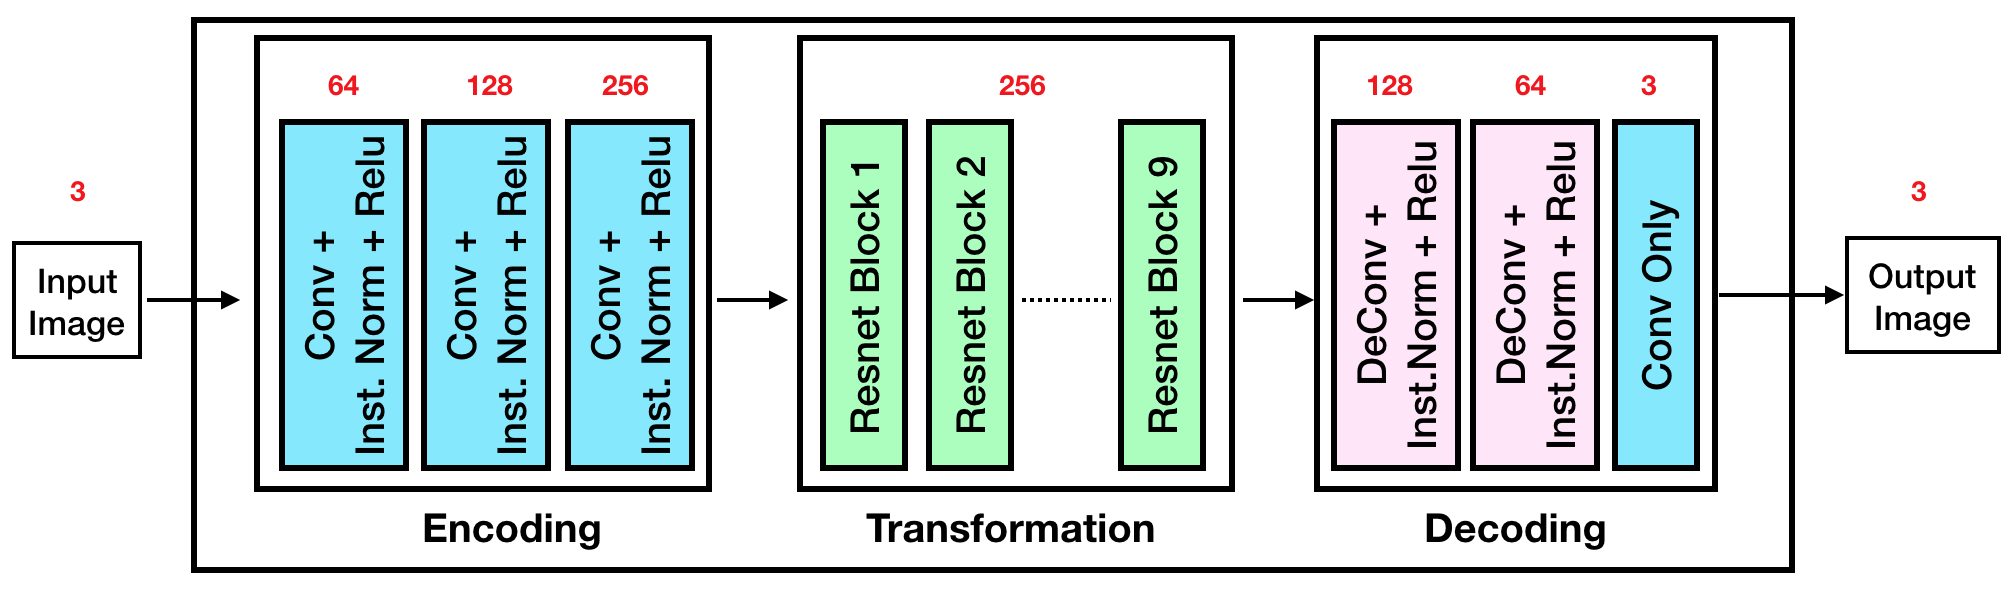
\includegraphics[width=\textwidth]{generator}
%         \caption{Generator}
%         \label{fig:gen}
%     \end{subfigure}
%     \vfill
%     \begin{subfigure}[b]{0.6\textwidth}
%         \centering
%         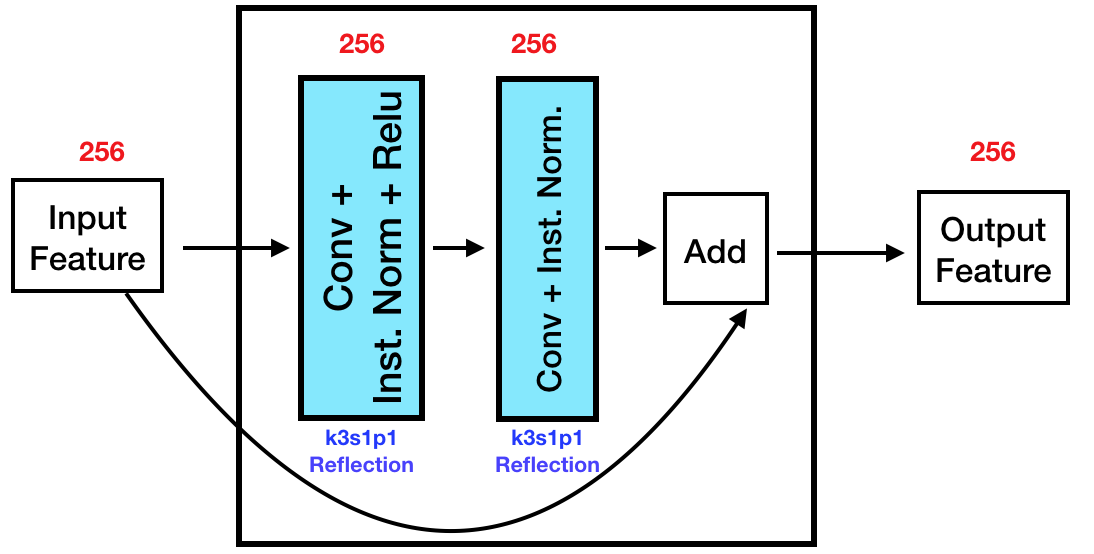
\includegraphics[width=\textwidth]{res_block}
%         \caption{Resnet Block in Detail}
%         \label{fig:res}
%     \end{subfigure}
%     \vfill
%     \begin{subfigure}[b]{0.8\textwidth}
%         \centering
%         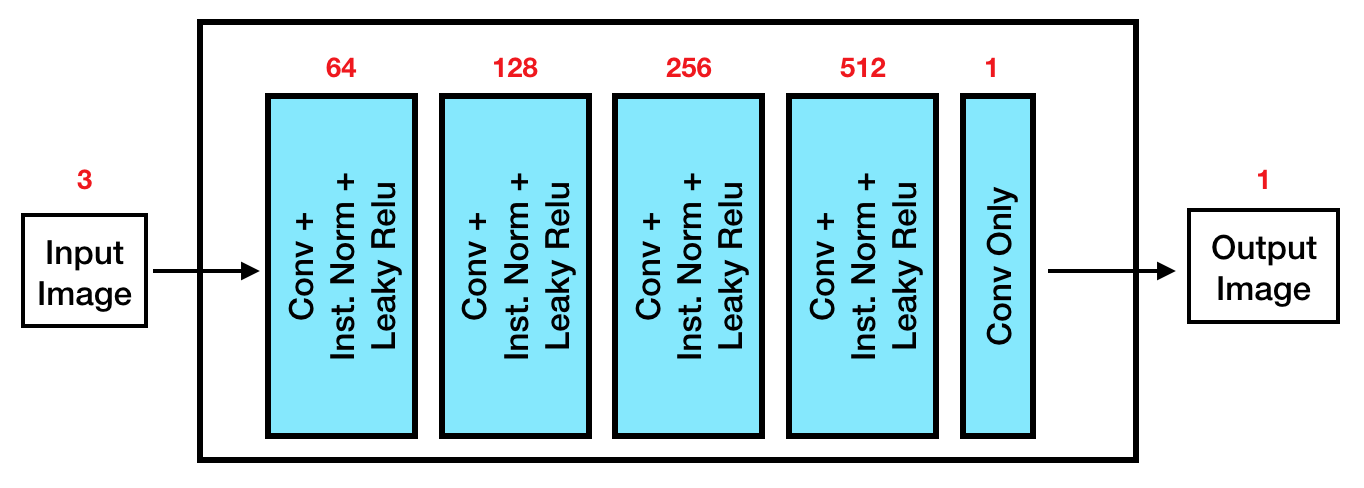
\includegraphics[width=\textwidth]{discriminator}
%         \caption{Discriminator}
%         \label{fig:disc}
%     \end{subfigure}
%        \caption{Network Architecture. The numbers in red refers to the number of output channels of each block. The letter-number combination in blue in form k\textit{x}s\textit{y}p\textit{z} beneath the blocks corresponds to the kernel size ($x$), stride ($y$) and padding ($z$). For example, k4s2p1 would mean a kernel size of $4 \times 4$, stride of 1 and padding of 1. If the padding is form $z-z$ , that means that a padding of $z$ is applied to the output as well (in addition to the input padding of $z$). The use of reflection padding has been indicated by the word Reflection in blue}
%        \label{fig:architecture}
%\end{figure*} 

\begin{figure*}[!htb]
     \centering
     \begin{subfigure}[]{0.49\textwidth}
         \centering
         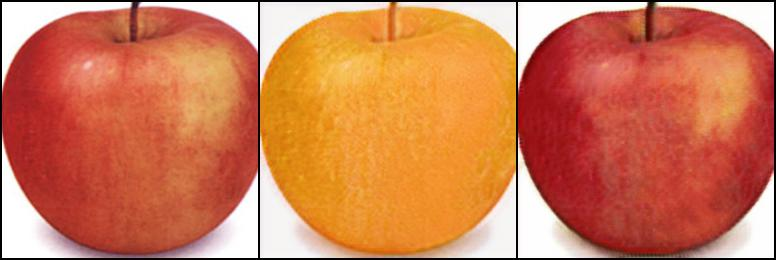
\includegraphics[width=0.9\textwidth]{test_a_2_b_32}\\
         \vspace{0.3cm}
		 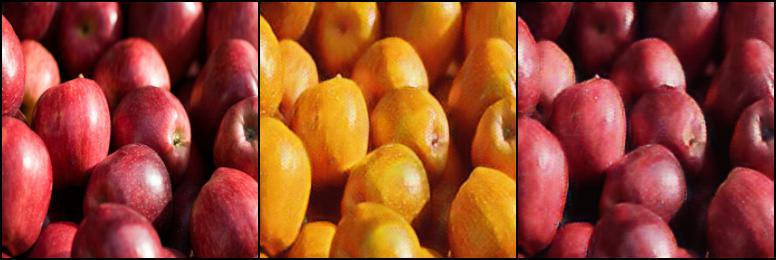
\includegraphics[width=0.9\textwidth]{test_a_2_b_65}\\
		 \vspace{0.3cm}
		 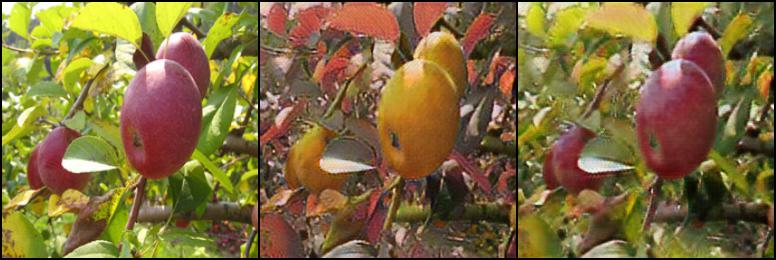
\includegraphics[width=0.9\textwidth]{test_a_2_b_111}
		 \caption{$Apple \rightarrow Orange \rightarrow Apple$}
         \label{fig:apple2orange}
     \end{subfigure}
     ~
     \begin{subfigure}[]{0.49\textwidth}
         \centering
         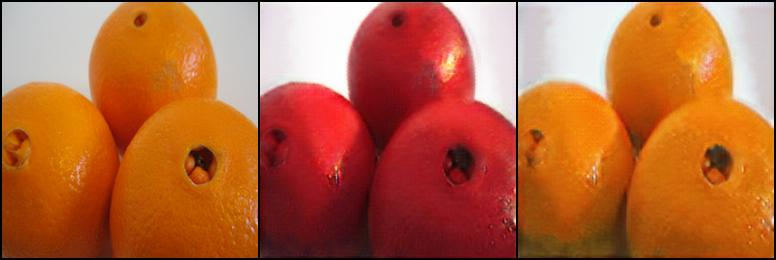
\includegraphics[width=0.9\textwidth]{test_b_2_a_46}\\
         \vspace{0.3cm}
		 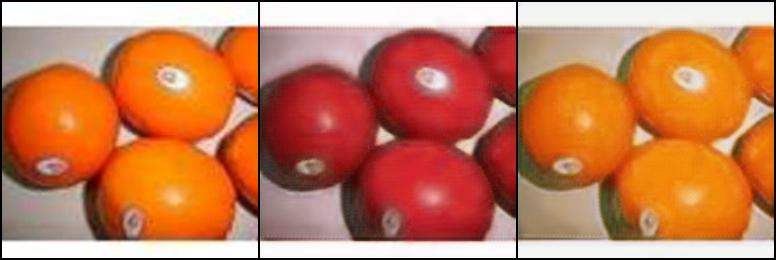
\includegraphics[width=0.9\textwidth]{test_b_2_a_214}\\
		 \vspace{0.3cm}
		 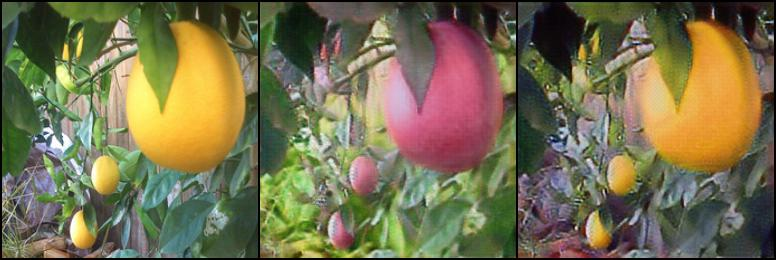
\includegraphics[width=0.9\textwidth]{test_b_2_a_243}
		 \caption{$Orange \rightarrow Apple \rightarrow Orange$}
         \label{fig:orange2apple}
     \end{subfigure}

     \caption{$Apple \leftrightarrow Orange$}
     \label{fig:orange22apple}
\end{figure*} 

\begin{figure*}[!htb]
     \centering
     \begin{subfigure}[]{0.49\textwidth}
         \centering
         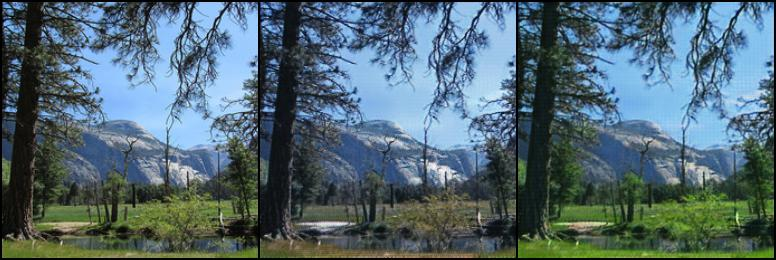
\includegraphics[width=0.9\textwidth]{test_a_2_b_111(1)}\\
         \vspace{0.3cm}
		 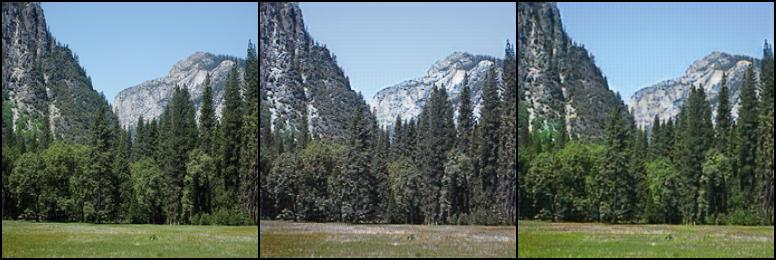
\includegraphics[width=0.9\textwidth]{test_a_2_b_63}\\
		 \vspace{0.3cm}
		 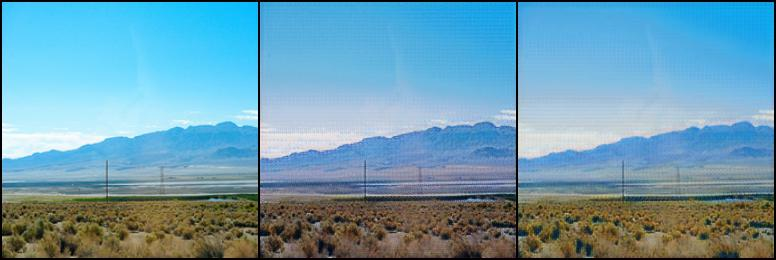
\includegraphics[width=0.9\textwidth]{test_a_2_b_220}
		 \caption{$Summer \rightarrow Winter \rightarrow Summer$}
         \label{fig:summer2winter}
     \end{subfigure}
     ~
     \begin{subfigure}[]{0.49\textwidth}
         \centering
         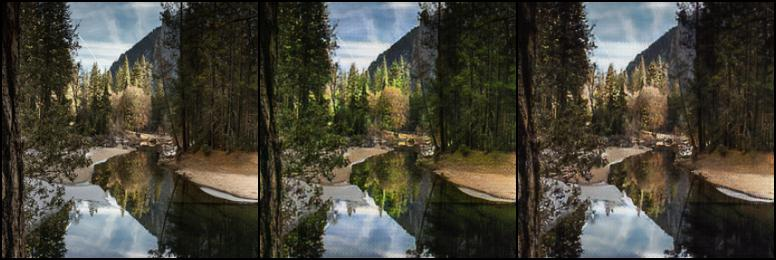
\includegraphics[width=0.9\textwidth]{test_b_2_a_132}\\
         \vspace{0.3cm}
		 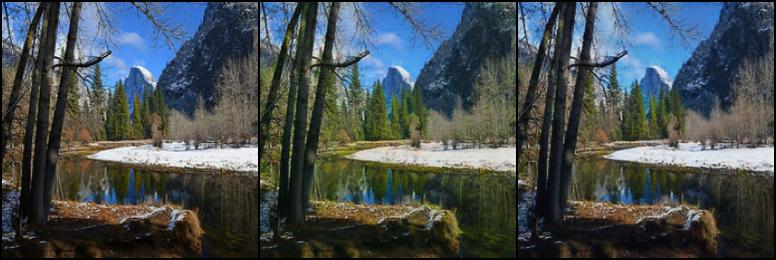
\includegraphics[width=0.9\textwidth]{test_b_2_a_168}\\
		 \vspace{0.3cm}
		 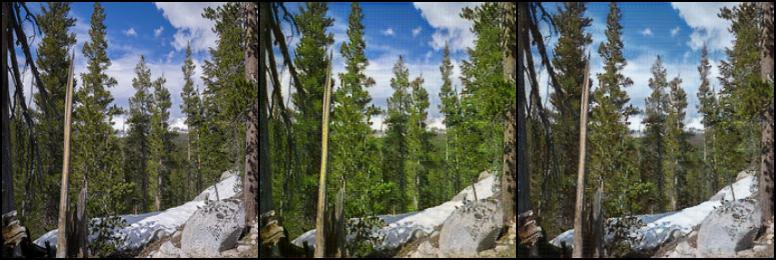
\includegraphics[width=0.9\textwidth]{test_b_2_a_211}
		 \caption{$Winter \rightarrow Summer \rightarrow Winter$}
         \label{fig:winter2summer}
     \end{subfigure}

     \caption{$Summer \leftrightarrow Winter$}
     \label{fig:summer22winter}
\end{figure*} 

\begin{figure*}[!htb]
     \centering
     \begin{subfigure}[]{0.49\textwidth}
         \centering
         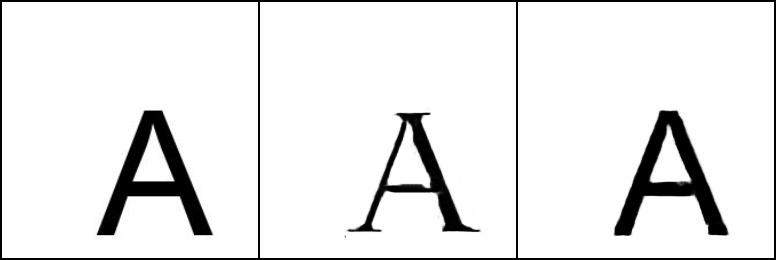
\includegraphics[width=0.9\textwidth]{test_a_2_b_4}\\
         \vspace{0.3cm}
		 
\includegraphics[width=0.9\textwidth]{test_a_2_b_32(1)}\\
		 \vspace{0.3cm}
		 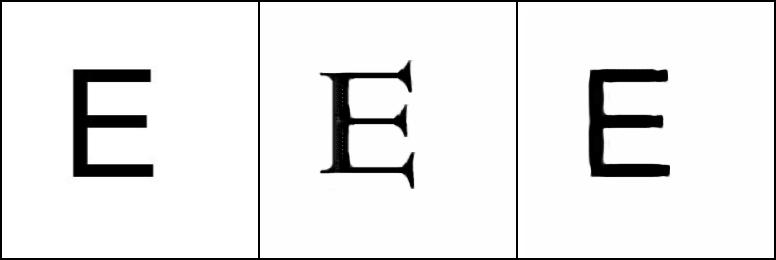
\includegraphics[width=0.9\textwidth]{test_a_2_b_40}\\
%		 \vspace{0.3cm}
%		 
\includegraphics[width=0.9\textwidth]{test_a_2_b_145}\\
%		 \vspace{0.3cm}
%		 
\includegraphics[width=0.9\textwidth]{test_a_2_b_206}
		 \caption{$Arial \rightarrow Times \rightarrow Arial$}
         \label{fig:arial2times}
     \end{subfigure}
     ~
     \begin{subfigure}[]{0.49\textwidth}
         \centering
         
\includegraphics[width=0.9\textwidth]{test_b_2_a_94}\\
         \vspace{0.3cm}
		 
\includegraphics[width=0.9\textwidth]{test_b_2_a_117}\\
		 \vspace{0.3cm}
		 
\includegraphics[width=0.9\textwidth]{test_b_2_a_136}\\
%		 \vspace{0.3cm}
%		 
\includegraphics[width=0.9\textwidth]{test_b_2_a_160}\\
%		 \vspace{0.3cm}
%		 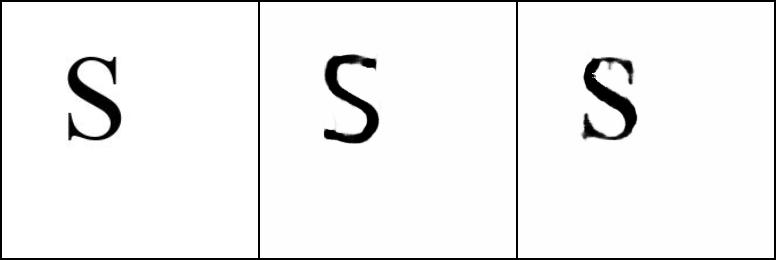
\includegraphics[width=0.9\textwidth]{test_b_2_a_171}
		 \caption{$Times \rightarrow Arial \rightarrow Times$}
         \label{fig:times2arial}
     \end{subfigure}

     \caption{$Arial \leftrightarrow Times$}
     \label{fig:arial22times}
\end{figure*} 

\begin{figure*}[!htb]
     \centering
     \begin{subfigure}[]{0.49\textwidth}
         \centering
         
\includegraphics[width=0.9\textwidth]{test_a_2_b_31}\\
         \vspace{0.3cm}
		 
\includegraphics[width=0.9\textwidth]{test_a_2_b_55}\\
		 \vspace{0.3cm}
		 
\includegraphics[width=0.9\textwidth]{test_a_2_b_341}\\
%		 \vspace{0.3cm}
%		 
\includegraphics[width=0.9\textwidth]{test_a_2_b_385}\\
%		 \vspace{0.3cm}
%		 
\includegraphics[width=0.9\textwidth]{test_a_2_b_490}
		 \caption{$Arial$ word $\rightarrow Times$ word$\rightarrow Arial$ word}
         \label{fig:arial2times_word}
     \end{subfigure}
     ~
     \begin{subfigure}[]{0.49\textwidth}
         \centering
         
\includegraphics[width=0.9\textwidth]{test_b_2_a_202}\\
         \vspace{0.3cm}
		 
\includegraphics[width=0.9\textwidth]{test_b_2_a_420}\\
		 \vspace{0.3cm}
		 
\includegraphics[width=0.9\textwidth]{test_b_2_a_436}\\
%		 \vspace{0.3cm}
%		 
\includegraphics[width=0.9\textwidth]{test_b_2_a_473}\\
%		 \vspace{0.3cm}
%		 
\includegraphics[width=0.9\textwidth]{test_b_2_a_492}
		 \caption{$Times$ word $\rightarrow Arial$ word$\rightarrow Times$ word}
         \label{fig:times2arial_word}
     \end{subfigure}

     \caption{$Arial$ word $\leftrightarrow Times$ word}
     \label{fig:arial22times_word}
\end{figure*} 

\begin{figure*}[!htb]
     \centering
     \begin{subfigure}[]{0.49\textwidth}
         \centering
         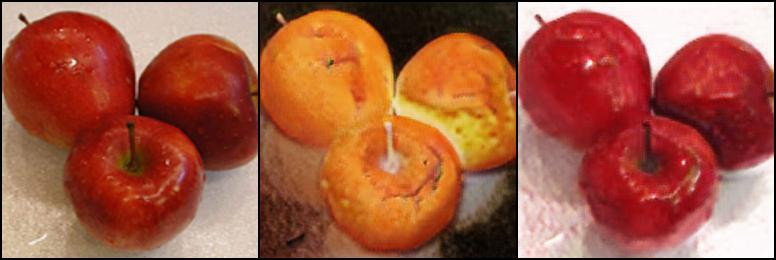
\includegraphics[width=0.9\textwidth]{test_a_2_b_33_i}\\
         \vspace{0.3cm}
		 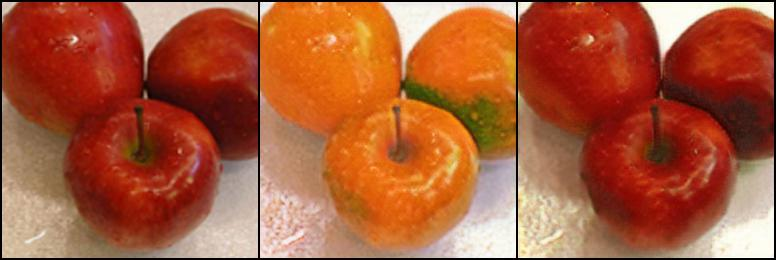
\includegraphics[width=0.9\textwidth]{test_a_2_b_33}\\
		 \caption{Learning rate 0.0002 (above) and 0.0004 (below)}
         \label{fig:a2r_lr}
     \end{subfigure}
     ~
     \begin{subfigure}[]{0.49\textwidth}
         \centering
         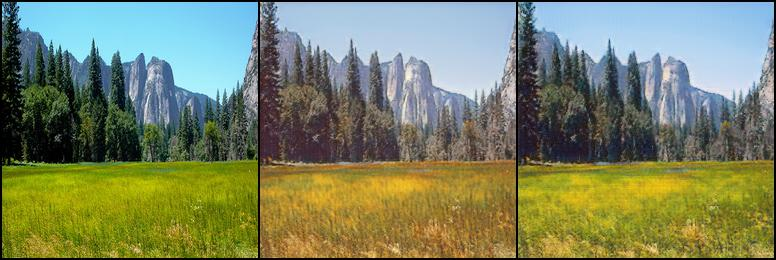
\includegraphics[width=0.9\textwidth]{test_a_2_b_48}\\
         \vspace{0.3cm}
		 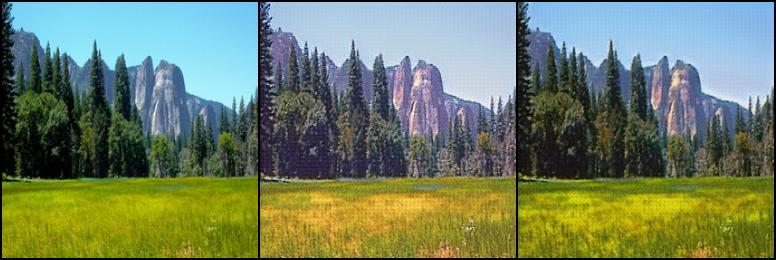
\includegraphics[width=0.9\textwidth]{test_a_2_b_48_g}\\
		 \caption{Identity loss not included (above) and included (below)}
         \label{fig:s2w_id}
     \end{subfigure}

     \caption{Learning Rate and Identity loss ablation for $Apple \leftrightarrow Orange$ and $Summer \leftrightarrow Winter$}
     \label{fig:ablation1}
\end{figure*} 

\begin{figure*}[!htb]
     \centering
     \begin{subfigure}[]{0.49\textwidth}
         \centering
         
\includegraphics[width=0.9\textwidth]{test_a_2_b_96}\\
         \vspace{0.3cm}
		 
\includegraphics[width=0.9\textwidth]{test_a_2_b_96_g}\\
		 \caption{Learning rate 0.0004 (above) and 0.0002 (below)}
         \label{fig:a2f_lr}
     \end{subfigure}
     ~
     \begin{subfigure}[]{0.49\textwidth}
         \centering
         
\includegraphics[width=0.9\textwidth]{test_a_2_b_115}\\
         \vspace{0.3cm}
		 
\includegraphics[width=0.9\textwidth]{test_a_2_b_115_g}\\
		 \caption{Identity loss not included (above) and included (below)}
         \label{fig:a2f_id}
     \end{subfigure}

     \caption{Learning Rate and Identity loss ablation for $Arial \leftrightarrow Times$}
     \label{fig:ablation2}
\end{figure*} 

\begin{figure*}[!htb]
     \centering
     \begin{subfigure}[]{0.49\textwidth}
         \centering
         
\includegraphics[width=0.9\textwidth]{test_a_2_b_203}\\
         \vspace{0.3cm}
		 
\includegraphics[width=0.9\textwidth]{test_a_2_b_203_g}\\
		 \caption{Learning rate 0.0004 (above) and 0.0002 (below)}
         \label{fig:a2f_w_lr}
     \end{subfigure}
     ~
     \begin{subfigure}[]{0.49\textwidth}
         \centering
         
\includegraphics[width=0.9\textwidth]{test_b_2_a_68}\\
         \vspace{0.3cm}
		 
\includegraphics[width=0.9\textwidth]{test_b_2_a_68_g}\\
		 \caption{Identity loss not included (above) and included (below)}
         \label{fig:a2f_w_id}
     \end{subfigure}

     \caption{Learning Rate and Identity loss ablation for $Arial \, word \leftrightarrow Times \, word$}
     \label{fig:ablation3}
\end{figure*}

Notice that both the generator and the discriminator networks are end-to-end fully convolutional. Before 
feeding our images to these networks, we resize them to $256 \times 256$. The output size of the generator network would be of the same size as it's input ($256 \times 256 \times 3$). The output of the 
discriminator is just a one single channel $30 \times 30$ feature map, which is compared against a $30 \times 30$ all 1's or all 0's tensor while calculating discriminator loss.

\section{Experimentation}

\subsection{Training}
We train our networks on a GeForce 1080 GPU using the training data collected for $summer2winter$ and $apple2orange$, and also using the generated training data for our
font style transfer. The original authors \cite{cyclegan} used 200 epochs and a learning rate of 0.0002, exponentially decaying the rate after first 100 epochs. We found after 
quite a bit of experimentation that for the $apple \leftrightarrow orange$ and $summer \leftrightarrow winter$ cases, the networks effectively cease to learn after 50 - 60 epochs, so we train these for 50 epochs only, exponentially decaying the learning rate after 25 epochs. We do the same for the font style transfer for full words. However, for the single character font style transfer, given that we have less training data, we use 100 epochs, exponentially decaying the learning rate after 50 epochs. We use Adam optimizer and a batch size of 1. We initialize the weights with a Normal distribution with mean 0 and standard deviation of 0.02. Table \ref{table:train} shows a summary of the training times. The supplementary document shows the trend of losses
over epochs for the generator loss, cycle-consistency loss, identity loss and discriminator loss.

\begin{table}[ht!]  
\begin{center}
\begin{tabular}{ |c|c|c| } 
 \hline
 \textbf{Domain} & \textbf{Epochs} & \textbf{Training Time} \\ 
 \hline
 $Apple \leftrightarrow Orange$ & 50 & 5 hours \\ 
 \hline
 $Summer \leftrightarrow Winter$ & 50 & 5 hours \\ 
 \hline
 $Arial \leftrightarrow Times$ & 100 & 3 hours \\ 
 \hline
 $Arial \, word\leftrightarrow Times \, word$ & 50 & 3.5 hours \\ 
 \hline
\end{tabular}
\end{center}
\caption{Training Times for different domains}
\label{table:train}
\end{table}

\subsection{Evaluation}
This is a kind of problem where the visual perception is a gold standard for
evaluating the quality of the translated images. Although a rigorous way of evaluating the quality of our images could have been using 
Amazon Mechanical Turk (AMT), due to our time constraints, we leave the quality
evaluation to the visual perception of ourselves and the readers. Figures 
\ref{fig:apple2orange} and \ref{fig:summer22winter} show some sample results of 
the $apple \leftrightarrow orange$ and $summer \leftrightarrow winter$ transfers. While 
the results are not extremely impressive, they do give the impression of real transfers to some extent.

We show some of our single character font style transfer results in Figure \
\ref{fig:arial22times} and some of our full word font style transfer results in
Figure \ref{fig:arial2times_word}. We see that although according to the original paper 
\cite{cyclegan}, the generators of CycleGAN was engineered for good performance on the appearance changes and not the shape changes in particular, it is capturing the shape changes of the fonts reasonably nicely. 

\subsection{Ablation}
We perform ablation studies separately on different domains. The main parameters we use for our ablation studies are number of epochs, learning rate, weight of the \textit{cycle-consistency loss} $\lambda$ and use of the \textit{identity loss}.

\subsubsection{$\mathbf{Apple \leftrightarrow Orange}$}
\noindent\textbf{Number of epochs} We tried varying number of epochs as 200, 100 and 50. We found that number of epochs more than 
50 does not really help, and the networks seem to be not learning much after that. We decided to keep it to 50. 

\noindent\textbf{Learning Rate} We found that using a rate of 0.0002 sometimes possibly gets trapped in a local minima and the network starts learning to invert the images for the first transformation, as if it is looking for a shortcut to get back to the original image via the cyclic transformation. Figure \ref{fig:a2r_lr} demonstrates this.

\noindent\textbf{Cycle-consistency weight $\lambda$ and Identity weight $\beta$} We tried with $\lambda$
values of 10 and 5, and for this case 5 turned out to work better. With 10, we get a similar local minima-like inverted phenomena that we discussed above for the low learning rate. For $\beta$, we tried 
with values 0 (exclude altogether) and 5, and 0 gave us better results.

\subsubsection{$\mathbf{Summer \leftrightarrow Winter}$}
\noindent\textbf{Number of epochs} Similarly for the $Apple \leftrightarrow Orange$ case, 50 turned out to be sufficient.

\noindent\textbf{Learning Rate} For this case, a learning rate of 0.0002 gave us slightly better results than 0.0004.

\noindent\textbf{Cycle-consistency weight $\lambda$ and Identity weight $\beta$} Again, we tried with 
$\lambda$ values of 10 and 5, and for this case 10 turned out to work better. For $\beta$, we tried 
with values 0 (exclude altogether) and 5, and 1 gave us better results. Just as the original authors \cite{cyclegan} had noticed, without the identity loss it changes the tint of the image a little bit. Figure \ref{fig:s2w_id} demonstrates this. 

\subsubsection{Font Style Transfer}
\noindent\textbf{Number of epochs} For single character uppercase $Arial \leftrightarrow Times$, we settle for an epoch number of 100, while for the full word transfer, we settle for 50.

\noindent\textbf{Learning Rate} Again for this case, a learning rate of 0.0002 gave us slightly better results than 0.0004 as shown in Figurer \ref{fig:a2f_lr} and \ref{fig:a2f_w_lr}.

\noindent\textbf{Cycle-consistency weight $\lambda$ and Identity weight $\beta$} Again, we tried with 
$\lambda$ values of 10 and 5, and for this case 10 turned out to work better. For $\beta$, including it (value 5) gave us slightly better results than excluding it as demonstrated in Figures \ref{fig:a2f_id} and \ref{fig:a2f_w_id}.
%-------------------------------------------------------------------------

\section{Conclusion and Future Work}

In this paper, we have tried to regenerate CycleGAN \cite{cyclegan} from scratch, explore two of the already explored domains and finally apply it to font style transfer
for single character and full words. We couldn't replicate all the possible domains
and results that the original paper did because of time constraints. From the results
we got, the attempt of applying it to font style transfer did look promising to some extent.
However, there is still quite a lot of ablations and tunings that can be done - like possibly modifying
the network architecture, using a different number of residual blocks (we used 9), trying out loss 
functions other than $L_2$ and $L_1$ norms, trying out batch and group normalizations instead of instance 
normalization etc. Also, our font and word images were all simple
black ones with a plain white background, while real world posters and artistic drawings would
contain fonts and backgrounds with varying colors and gradients, which is a definitely challenge
to explore in the future.

\noindent \textbf{Acknowledgements} Dr. Kosta Derpanis and Matthew Kowal.

{\small
\bibliographystyle{ieee}
\bibliography{egbib}
}

\end{document}
